% Created by tikzDevice version 0.12.6 on 2026-03-25 09:34:47
% !TEX encoding = UTF-8 Unicode
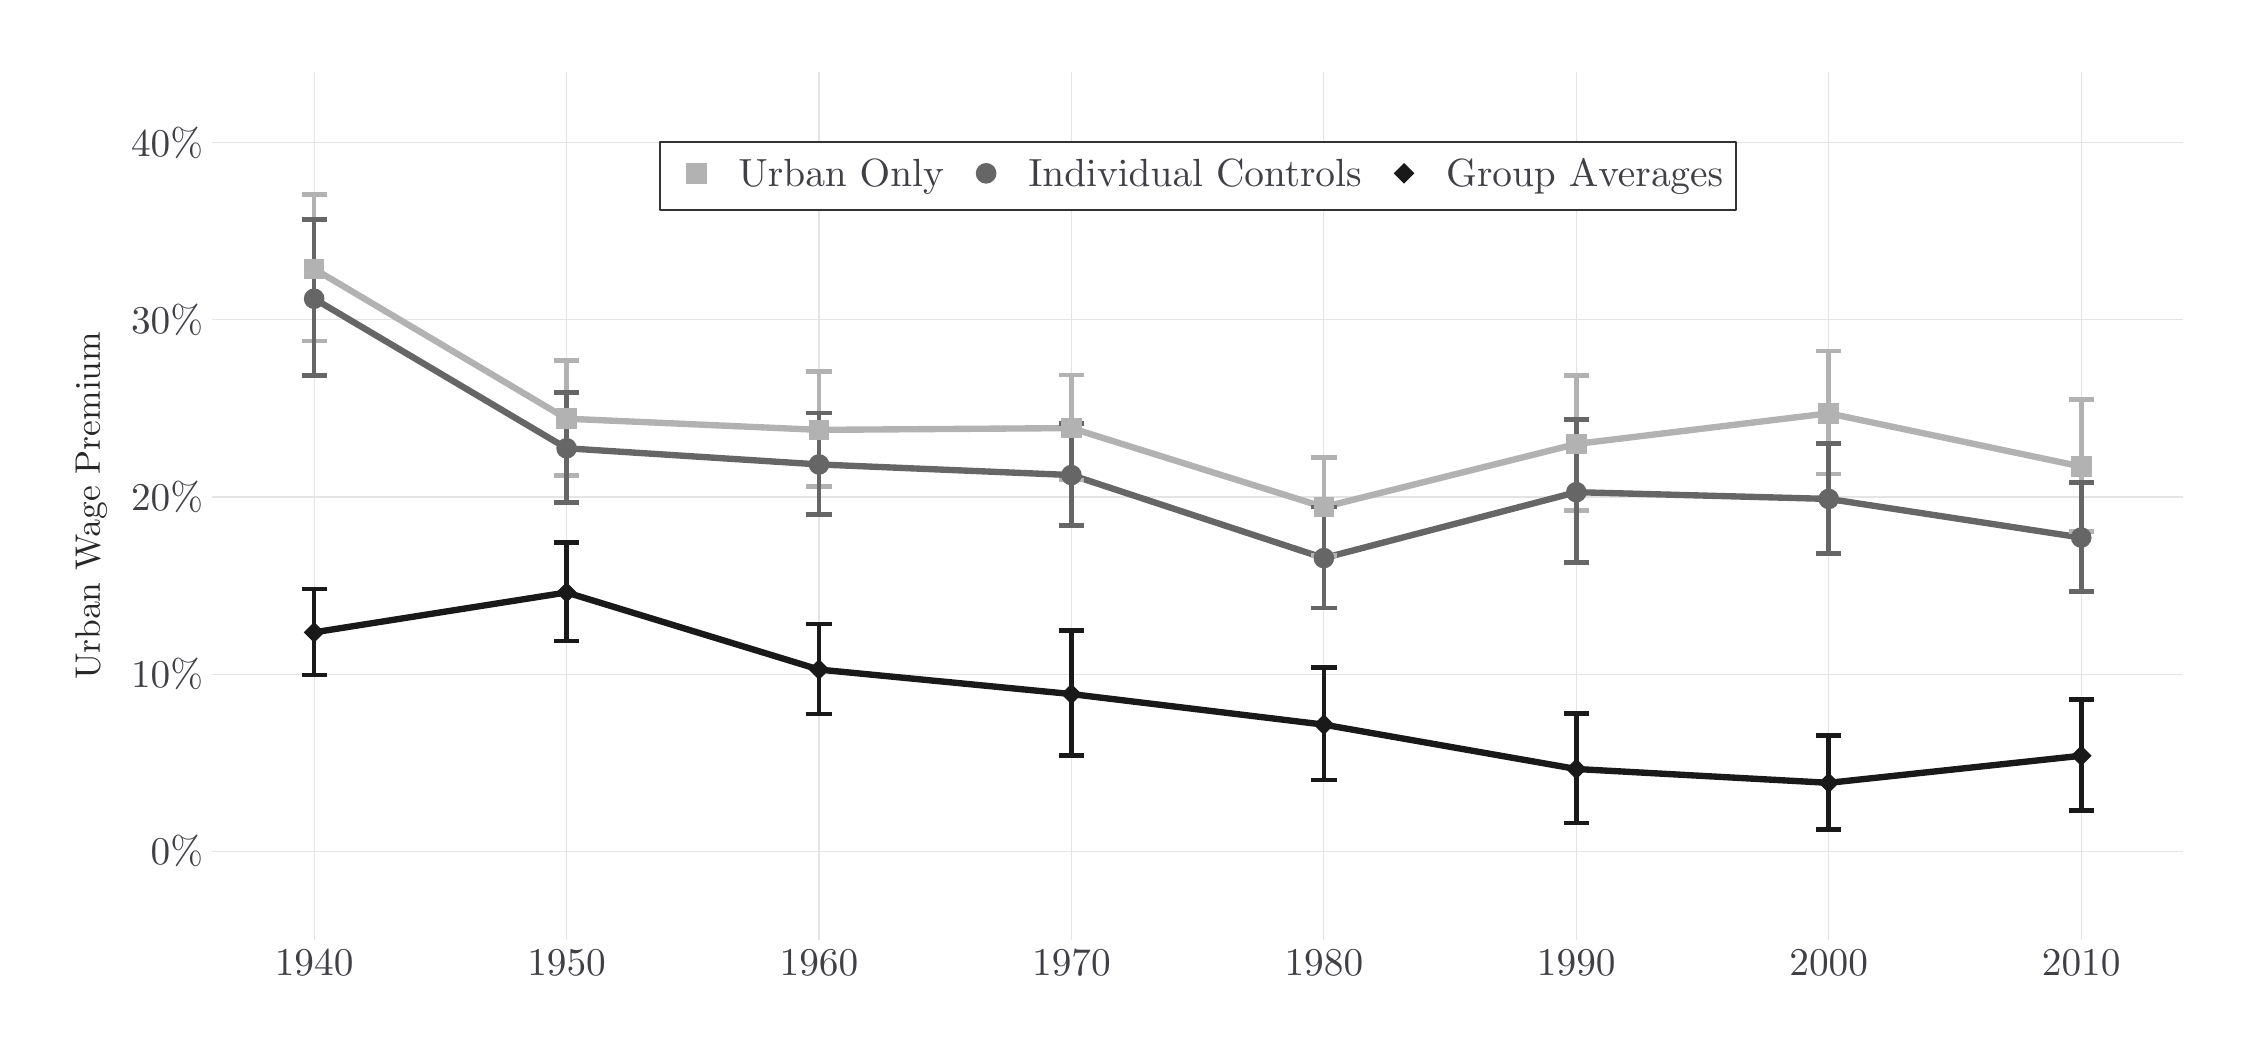
\begin{tikzpicture}[x=1pt,y=1pt]
\definecolor{fillColor}{RGB}{255,255,255}
\path[use as bounding box,fill=fillColor] (0,0) rectangle (794.97,361.35);
\begin{scope}
\path[clip] (  0.00,  0.00) rectangle (794.97,361.35);
\definecolor{drawColor}{RGB}{255,255,255}

\path[draw=drawColor,line width= 0.8pt,line join=round,line cap=round,fill=fillColor] (  0.00,  0.00) rectangle (794.97,361.35);
\end{scope}
\begin{scope}
\path[clip] ( 66.57, 31.76) rectangle (778.97,345.35);
\definecolor{drawColor}{RGB}{255,255,255}
\definecolor{fillColor}{RGB}{255,255,255}

\path[draw=drawColor,line width= 0.8pt,line join=round,line cap=round,fill=fillColor] ( 66.57, 31.76) rectangle (778.97,345.35);
\definecolor{drawColor}{RGB}{228,228,231}

\path[draw=drawColor,line width= 0.4pt,line join=round] ( 66.57, 63.76) --
	(778.97, 63.76);

\path[draw=drawColor,line width= 0.4pt,line join=round] ( 66.57,127.76) --
	(778.97,127.76);

\path[draw=drawColor,line width= 0.4pt,line join=round] ( 66.57,191.75) --
	(778.97,191.75);

\path[draw=drawColor,line width= 0.4pt,line join=round] ( 66.57,255.75) --
	(778.97,255.75);

\path[draw=drawColor,line width= 0.4pt,line join=round] ( 66.57,319.75) --
	(778.97,319.75);

\path[draw=drawColor,line width= 0.4pt,line join=round] (103.51, 31.76) --
	(103.51,345.35);

\path[draw=drawColor,line width= 0.4pt,line join=round] (194.73, 31.76) --
	(194.73,345.35);

\path[draw=drawColor,line width= 0.4pt,line join=round] (285.94, 31.76) --
	(285.94,345.35);

\path[draw=drawColor,line width= 0.4pt,line join=round] (377.16, 31.76) --
	(377.16,345.35);

\path[draw=drawColor,line width= 0.4pt,line join=round] (468.38, 31.76) --
	(468.38,345.35);

\path[draw=drawColor,line width= 0.4pt,line join=round] (559.59, 31.76) --
	(559.59,345.35);

\path[draw=drawColor,line width= 0.4pt,line join=round] (650.81, 31.76) --
	(650.81,345.35);

\path[draw=drawColor,line width= 0.4pt,line join=round] (742.03, 31.76) --
	(742.03,345.35);
\definecolor{drawColor}{gray}{0.70}

\path[draw=drawColor,line width= 2.3pt,line join=round] (103.51,274.18) --
	(194.73,220.06) --
	(285.94,216.01) --
	(377.16,216.65) --
	(468.38,188.10) --
	(559.59,210.92) --
	(650.81,221.99) --
	(742.03,202.77);
\definecolor{drawColor}{gray}{0.40}

\path[draw=drawColor,line width= 2.3pt,line join=round] (103.51,263.40) --
	(194.73,209.36) --
	(285.94,203.52) --
	(377.16,199.68) --
	(468.38,169.68) --
	(559.59,193.50) --
	(650.81,191.06) --
	(742.03,177.10);
\definecolor{drawColor}{gray}{0.10}

\path[draw=drawColor,line width= 2.3pt,line join=round] (103.51,142.85) --
	(194.73,157.26) --
	(285.94,129.40) --
	(377.16,120.55) --
	(468.38,109.50) --
	(559.59, 93.47) --
	(650.81, 88.47) --
	(742.03, 98.26);
\definecolor{drawColor}{gray}{0.70}

\path[draw=drawColor,line width= 1.7pt,line join=round] ( 98.95,301.04) --
	(108.07,301.04);

\path[draw=drawColor,line width= 1.7pt,line join=round] (103.51,301.04) --
	(103.51,248.14);

\path[draw=drawColor,line width= 1.7pt,line join=round] ( 98.95,248.14) --
	(108.07,248.14);
\definecolor{drawColor}{gray}{0.40}

\path[draw=drawColor,line width= 1.7pt,line join=round] ( 98.95,292.00) --
	(108.07,292.00);

\path[draw=drawColor,line width= 1.7pt,line join=round] (103.51,292.00) --
	(103.51,235.73);

\path[draw=drawColor,line width= 1.7pt,line join=round] ( 98.95,235.73) --
	(108.07,235.73);
\definecolor{drawColor}{gray}{0.10}

\path[draw=drawColor,line width= 1.7pt,line join=round] ( 98.95,158.56) --
	(108.07,158.56);

\path[draw=drawColor,line width= 1.7pt,line join=round] (103.51,158.56) --
	(103.51,127.47);

\path[draw=drawColor,line width= 1.7pt,line join=round] ( 98.95,127.47) --
	(108.07,127.47);
\definecolor{drawColor}{gray}{0.70}

\path[draw=drawColor,line width= 1.7pt,line join=round] (190.17,241.06) --
	(199.29,241.06);

\path[draw=drawColor,line width= 1.7pt,line join=round] (194.73,241.06) --
	(194.73,199.61);

\path[draw=drawColor,line width= 1.7pt,line join=round] (190.17,199.61) --
	(199.29,199.61);
\definecolor{drawColor}{gray}{0.40}

\path[draw=drawColor,line width= 1.7pt,line join=round] (190.17,229.52) --
	(199.29,229.52);

\path[draw=drawColor,line width= 1.7pt,line join=round] (194.73,229.52) --
	(194.73,189.71);

\path[draw=drawColor,line width= 1.7pt,line join=round] (190.17,189.71) --
	(199.29,189.71);
\definecolor{drawColor}{gray}{0.10}

\path[draw=drawColor,line width= 1.7pt,line join=round] (190.17,175.27) --
	(199.29,175.27);

\path[draw=drawColor,line width= 1.7pt,line join=round] (194.73,175.27) --
	(194.73,139.68);

\path[draw=drawColor,line width= 1.7pt,line join=round] (190.17,139.68) --
	(199.29,139.68);
\definecolor{drawColor}{gray}{0.70}

\path[draw=drawColor,line width= 1.7pt,line join=round] (281.38,236.98) --
	(290.50,236.98);

\path[draw=drawColor,line width= 1.7pt,line join=round] (285.94,236.98) --
	(285.94,195.58);

\path[draw=drawColor,line width= 1.7pt,line join=round] (281.38,195.58) --
	(290.50,195.58);
\definecolor{drawColor}{gray}{0.40}

\path[draw=drawColor,line width= 1.7pt,line join=round] (281.38,222.16) --
	(290.50,222.16);

\path[draw=drawColor,line width= 1.7pt,line join=round] (285.94,222.16) --
	(285.94,185.31);

\path[draw=drawColor,line width= 1.7pt,line join=round] (281.38,185.31) --
	(290.50,185.31);
\definecolor{drawColor}{gray}{0.10}

\path[draw=drawColor,line width= 1.7pt,line join=round] (281.38,145.87) --
	(290.50,145.87);

\path[draw=drawColor,line width= 1.7pt,line join=round] (285.94,145.87) --
	(285.94,113.32);

\path[draw=drawColor,line width= 1.7pt,line join=round] (281.38,113.32) --
	(290.50,113.32);
\definecolor{drawColor}{gray}{0.70}

\path[draw=drawColor,line width= 1.7pt,line join=round] (372.60,235.86) --
	(381.72,235.86);

\path[draw=drawColor,line width= 1.7pt,line join=round] (377.16,235.86) --
	(377.16,197.89);

\path[draw=drawColor,line width= 1.7pt,line join=round] (372.60,197.89) --
	(381.72,197.89);
\definecolor{drawColor}{gray}{0.40}

\path[draw=drawColor,line width= 1.7pt,line join=round] (372.60,218.41) --
	(381.72,218.41);

\path[draw=drawColor,line width= 1.7pt,line join=round] (377.16,218.41) --
	(377.16,181.39);

\path[draw=drawColor,line width= 1.7pt,line join=round] (372.60,181.39) --
	(381.72,181.39);
\definecolor{drawColor}{gray}{0.10}

\path[draw=drawColor,line width= 1.7pt,line join=round] (372.60,143.48) --
	(381.72,143.48);

\path[draw=drawColor,line width= 1.7pt,line join=round] (377.16,143.48) --
	(377.16, 98.35);

\path[draw=drawColor,line width= 1.7pt,line join=round] (372.60, 98.35) --
	(381.72, 98.35);
\definecolor{drawColor}{gray}{0.70}

\path[draw=drawColor,line width= 1.7pt,line join=round] (463.82,206.13) --
	(472.94,206.13);

\path[draw=drawColor,line width= 1.7pt,line join=round] (468.38,206.13) --
	(468.38,170.49);

\path[draw=drawColor,line width= 1.7pt,line join=round] (463.82,170.49) --
	(472.94,170.49);
\definecolor{drawColor}{gray}{0.40}

\path[draw=drawColor,line width= 1.7pt,line join=round] (463.82,188.14) --
	(472.94,188.14);

\path[draw=drawColor,line width= 1.7pt,line join=round] (468.38,188.14) --
	(468.38,151.67);

\path[draw=drawColor,line width= 1.7pt,line join=round] (463.82,151.67) --
	(472.94,151.67);
\definecolor{drawColor}{gray}{0.10}

\path[draw=drawColor,line width= 1.7pt,line join=round] (463.82,130.15) --
	(472.94,130.15);

\path[draw=drawColor,line width= 1.7pt,line join=round] (468.38,130.15) --
	(468.38, 89.46);

\path[draw=drawColor,line width= 1.7pt,line join=round] (463.82, 89.46) --
	(472.94, 89.46);
\definecolor{drawColor}{gray}{0.70}

\path[draw=drawColor,line width= 1.7pt,line join=round] (555.03,235.61) --
	(564.15,235.61);

\path[draw=drawColor,line width= 1.7pt,line join=round] (559.59,235.61) --
	(559.59,186.99);

\path[draw=drawColor,line width= 1.7pt,line join=round] (555.03,186.99) --
	(564.15,186.99);
\definecolor{drawColor}{gray}{0.40}

\path[draw=drawColor,line width= 1.7pt,line join=round] (555.03,219.84) --
	(564.15,219.84);

\path[draw=drawColor,line width= 1.7pt,line join=round] (559.59,219.84) --
	(559.59,168.03);

\path[draw=drawColor,line width= 1.7pt,line join=round] (555.03,168.03) --
	(564.15,168.03);
\definecolor{drawColor}{gray}{0.10}

\path[draw=drawColor,line width= 1.7pt,line join=round] (555.03,113.54) --
	(564.15,113.54);

\path[draw=drawColor,line width= 1.7pt,line join=round] (559.59,113.54) --
	(559.59, 73.99);

\path[draw=drawColor,line width= 1.7pt,line join=round] (555.03, 73.99) --
	(564.15, 73.99);
\definecolor{drawColor}{gray}{0.70}

\path[draw=drawColor,line width= 1.7pt,line join=round] (646.25,244.49) --
	(655.37,244.49);

\path[draw=drawColor,line width= 1.7pt,line join=round] (650.81,244.49) --
	(650.81,200.11);

\path[draw=drawColor,line width= 1.7pt,line join=round] (646.25,200.11) --
	(655.37,200.11);
\definecolor{drawColor}{gray}{0.40}

\path[draw=drawColor,line width= 1.7pt,line join=round] (646.25,211.17) --
	(655.37,211.17);

\path[draw=drawColor,line width= 1.7pt,line join=round] (650.81,211.17) --
	(650.81,171.46);

\path[draw=drawColor,line width= 1.7pt,line join=round] (646.25,171.46) --
	(655.37,171.46);
\definecolor{drawColor}{gray}{0.10}

\path[draw=drawColor,line width= 1.7pt,line join=round] (646.25,105.70) --
	(655.37,105.70);

\path[draw=drawColor,line width= 1.7pt,line join=round] (650.81,105.70) --
	(650.81, 71.68);

\path[draw=drawColor,line width= 1.7pt,line join=round] (646.25, 71.68) --
	(655.37, 71.68);
\definecolor{drawColor}{gray}{0.70}

\path[draw=drawColor,line width= 1.7pt,line join=round] (737.47,226.88) --
	(746.59,226.88);

\path[draw=drawColor,line width= 1.7pt,line join=round] (742.03,226.88) --
	(742.03,179.37);

\path[draw=drawColor,line width= 1.7pt,line join=round] (737.47,179.37) --
	(746.59,179.37);
\definecolor{drawColor}{gray}{0.40}

\path[draw=drawColor,line width= 1.7pt,line join=round] (737.47,197.00) --
	(746.59,197.00);

\path[draw=drawColor,line width= 1.7pt,line join=round] (742.03,197.00) --
	(742.03,157.70);

\path[draw=drawColor,line width= 1.7pt,line join=round] (737.47,157.70) --
	(746.59,157.70);
\definecolor{drawColor}{gray}{0.10}

\path[draw=drawColor,line width= 1.7pt,line join=round] (737.47,118.66) --
	(746.59,118.66);

\path[draw=drawColor,line width= 1.7pt,line join=round] (742.03,118.66) --
	(742.03, 78.46);

\path[draw=drawColor,line width= 1.7pt,line join=round] (737.47, 78.46) --
	(746.59, 78.46);
\definecolor{fillColor}{gray}{0.70}

\path[fill=fillColor] ( 99.78,270.45) --
	(107.24,270.45) --
	(107.24,277.91) --
	( 99.78,277.91) --
	cycle;
\definecolor{fillColor}{gray}{0.40}

\path[fill=fillColor] (103.51,263.40) circle (  3.73);
\definecolor{fillColor}{gray}{0.10}

\path[fill=fillColor] ( 99.78,142.85) --
	(103.51,146.58) --
	(107.24,142.85) --
	(103.51,139.12) --
	cycle;
\definecolor{fillColor}{gray}{0.70}

\path[fill=fillColor] (191.00,216.33) --
	(198.46,216.33) --
	(198.46,223.79) --
	(191.00,223.79) --
	cycle;
\definecolor{fillColor}{gray}{0.40}

\path[fill=fillColor] (194.73,209.36) circle (  3.73);
\definecolor{fillColor}{gray}{0.10}

\path[fill=fillColor] (191.00,157.26) --
	(194.73,160.99) --
	(198.46,157.26) --
	(194.73,153.53) --
	cycle;
\definecolor{fillColor}{gray}{0.70}

\path[fill=fillColor] (282.21,212.28) --
	(289.67,212.28) --
	(289.67,219.74) --
	(282.21,219.74) --
	cycle;
\definecolor{fillColor}{gray}{0.40}

\path[fill=fillColor] (285.94,203.52) circle (  3.73);
\definecolor{fillColor}{gray}{0.10}

\path[fill=fillColor] (282.21,129.40) --
	(285.94,133.13) --
	(289.67,129.40) --
	(285.94,125.67) --
	cycle;
\definecolor{fillColor}{gray}{0.70}

\path[fill=fillColor] (373.43,212.92) --
	(380.89,212.92) --
	(380.89,220.38) --
	(373.43,220.38) --
	cycle;
\definecolor{fillColor}{gray}{0.40}

\path[fill=fillColor] (377.16,199.68) circle (  3.73);
\definecolor{fillColor}{gray}{0.10}

\path[fill=fillColor] (373.43,120.55) --
	(377.16,124.28) --
	(380.89,120.55) --
	(377.16,116.82) --
	cycle;
\definecolor{fillColor}{gray}{0.70}

\path[fill=fillColor] (464.65,184.37) --
	(472.11,184.37) --
	(472.11,191.83) --
	(464.65,191.83) --
	cycle;
\definecolor{fillColor}{gray}{0.40}

\path[fill=fillColor] (468.38,169.68) circle (  3.73);
\definecolor{fillColor}{gray}{0.10}

\path[fill=fillColor] (464.65,109.50) --
	(468.38,113.23) --
	(472.11,109.50) --
	(468.38,105.77) --
	cycle;
\definecolor{fillColor}{gray}{0.70}

\path[fill=fillColor] (555.86,207.19) --
	(563.32,207.19) --
	(563.32,214.65) --
	(555.86,214.65) --
	cycle;
\definecolor{fillColor}{gray}{0.40}

\path[fill=fillColor] (559.59,193.50) circle (  3.73);
\definecolor{fillColor}{gray}{0.10}

\path[fill=fillColor] (555.86, 93.47) --
	(559.59, 97.21) --
	(563.32, 93.47) --
	(559.59, 89.74) --
	cycle;
\definecolor{fillColor}{gray}{0.70}

\path[fill=fillColor] (647.08,218.26) --
	(654.54,218.26) --
	(654.54,225.72) --
	(647.08,225.72) --
	cycle;
\definecolor{fillColor}{gray}{0.40}

\path[fill=fillColor] (650.81,191.06) circle (  3.73);
\definecolor{fillColor}{gray}{0.10}

\path[fill=fillColor] (647.08, 88.47) --
	(650.81, 92.20) --
	(654.54, 88.47) --
	(650.81, 84.74) --
	cycle;
\definecolor{fillColor}{gray}{0.70}

\path[fill=fillColor] (738.30,199.04) --
	(745.76,199.04) --
	(745.76,206.50) --
	(738.30,206.50) --
	cycle;
\definecolor{fillColor}{gray}{0.40}

\path[fill=fillColor] (742.03,177.10) circle (  3.73);
\definecolor{fillColor}{gray}{0.10}

\path[fill=fillColor] (738.30, 98.26) --
	(742.03,101.99) --
	(745.76, 98.26) --
	(742.03, 94.53) --
	cycle;
\end{scope}
\begin{scope}
\path[clip] (  0.00,  0.00) rectangle (794.97,361.35);
\definecolor{drawColor}{RGB}{63,63,70}

\node[text=drawColor,anchor=base east,inner sep=0pt, outer sep=0pt, scale=  1.42] at ( 63.37, 58.86) {0\%};

\node[text=drawColor,anchor=base east,inner sep=0pt, outer sep=0pt, scale=  1.42] at ( 63.37,122.86) {10\%};

\node[text=drawColor,anchor=base east,inner sep=0pt, outer sep=0pt, scale=  1.42] at ( 63.37,186.86) {20\%};

\node[text=drawColor,anchor=base east,inner sep=0pt, outer sep=0pt, scale=  1.42] at ( 63.37,250.86) {30\%};

\node[text=drawColor,anchor=base east,inner sep=0pt, outer sep=0pt, scale=  1.42] at ( 63.37,314.85) {40\%};
\end{scope}
\begin{scope}
\path[clip] (  0.00,  0.00) rectangle (794.97,361.35);
\definecolor{drawColor}{RGB}{63,63,70}

\node[text=drawColor,anchor=base,inner sep=0pt, outer sep=0pt, scale=  1.42] at (103.51, 18.76) {1940};

\node[text=drawColor,anchor=base,inner sep=0pt, outer sep=0pt, scale=  1.42] at (194.73, 18.76) {1950};

\node[text=drawColor,anchor=base,inner sep=0pt, outer sep=0pt, scale=  1.42] at (285.94, 18.76) {1960};

\node[text=drawColor,anchor=base,inner sep=0pt, outer sep=0pt, scale=  1.42] at (377.16, 18.76) {1970};

\node[text=drawColor,anchor=base,inner sep=0pt, outer sep=0pt, scale=  1.42] at (468.38, 18.76) {1980};

\node[text=drawColor,anchor=base,inner sep=0pt, outer sep=0pt, scale=  1.42] at (559.59, 18.76) {1990};

\node[text=drawColor,anchor=base,inner sep=0pt, outer sep=0pt, scale=  1.42] at (650.81, 18.76) {2000};

\node[text=drawColor,anchor=base,inner sep=0pt, outer sep=0pt, scale=  1.42] at (742.03, 18.76) {2010};
\end{scope}
\begin{scope}
\path[clip] (  0.00,  0.00) rectangle (794.97,361.35);
\definecolor{drawColor}{RGB}{39,39,42}

\node[text=drawColor,rotate= 90.00,anchor=base,inner sep=0pt, outer sep=0pt, scale=  1.28] at ( 26.06,188.55) {Urban Wage Premium};
\end{scope}
\begin{scope}
\path[clip] (  0.00,  0.00) rectangle (794.97,361.35);
\definecolor{drawColor}{gray}{0.20}
\definecolor{fillColor}{RGB}{255,255,255}

\path[draw=drawColor,line width= 0.8pt,line join=round,line cap=round,fill=fillColor] (228.37,295.49) rectangle (617.17,319.95);
\end{scope}
\begin{scope}
\path[clip] (  0.00,  0.00) rectangle (794.97,361.35);
\definecolor{drawColor}{RGB}{255,255,255}
\definecolor{fillColor}{RGB}{255,255,255}

\path[draw=drawColor,line width= 0.8pt,line join=round,line cap=round,fill=fillColor] (234.37,301.49) rectangle (248.83,315.95);
\definecolor{fillColor}{gray}{0.70}

\path[fill=fillColor] (237.87,304.99) --
	(245.33,304.99) --
	(245.33,312.45) --
	(237.87,312.45) --
	cycle;
\end{scope}
\begin{scope}
\path[clip] (  0.00,  0.00) rectangle (794.97,361.35);
\definecolor{drawColor}{RGB}{255,255,255}
\definecolor{fillColor}{RGB}{255,255,255}

\path[draw=drawColor,line width= 0.8pt,line join=round,line cap=round,fill=fillColor] (339.11,301.49) rectangle (353.56,315.95);
\definecolor{fillColor}{gray}{0.40}

\path[fill=fillColor] (346.33,308.72) circle (  3.73);
\end{scope}
\begin{scope}
\path[clip] (  0.00,  0.00) rectangle (794.97,361.35);
\definecolor{drawColor}{RGB}{255,255,255}
\definecolor{fillColor}{RGB}{255,255,255}

\path[draw=drawColor,line width= 0.8pt,line join=round,line cap=round,fill=fillColor] (490.12,301.49) rectangle (504.58,315.95);
\definecolor{fillColor}{gray}{0.10}

\path[fill=fillColor] (493.62,308.72) --
	(497.35,312.45) --
	(501.08,308.72) --
	(497.35,304.99) --
	cycle;
\end{scope}
\begin{scope}
\path[clip] (  0.00,  0.00) rectangle (794.97,361.35);
\definecolor{drawColor}{RGB}{63,63,70}

\node[text=drawColor,anchor=base west,inner sep=0pt, outer sep=0pt, scale=  1.42] at (256.83,303.82) {Urban Only};
\end{scope}
\begin{scope}
\path[clip] (  0.00,  0.00) rectangle (794.97,361.35);
\definecolor{drawColor}{RGB}{63,63,70}

\node[text=drawColor,anchor=base west,inner sep=0pt, outer sep=0pt, scale=  1.42] at (361.56,303.82) {Individual Controls};
\end{scope}
\begin{scope}
\path[clip] (  0.00,  0.00) rectangle (794.97,361.35);
\definecolor{drawColor}{RGB}{63,63,70}

\node[text=drawColor,anchor=base west,inner sep=0pt, outer sep=0pt, scale=  1.42] at (512.58,303.82) {Group Averages};
\end{scope}
\end{tikzpicture}
